\section{Ergebnisse}
\label{ergebnisse}

\subsection{Erkennungsrate}
\label{ergebnisse:erfolg}

Für die Bestimmung der Erkennungsrate der \textit{Inferenz} werden in den folgenden Abschnitten zwei \textit{Scores}
gebildet: der \textit{Wordscore} $W$ und der \textit{Charscore} $C$. $W$ ist ein binärer Wert und gibt an, ob ein ganzes
Wort korrekt erkannt wurde. $C$ errechnet sich aus der Anzahl der korrekt erkannten Buchstaben geteilt durch die
Gesamtzahl der Buchstaben des Wortes. Anders ausgedrückt bedeutet $W = 1$ immer $C = 1$; $C < 1$ impliziert immer
$W = 0$.

Beispiele:

\begin{itemize}
    \item Der Text \glqq Bramel\grqq\ wird korrekt als \glqq Bramel\grqq\ erkannt. $W = C = 1$
    \item Der Text \glqq Ta\textbf{\color{red}n}nen\grqq\ wird als \glqq Ta\textbf{\color{red}u}nen\grqq\ erkannt.
          $W = 0$, $C = 0,8333$
\end{itemize}

Dieses Verfahren erlaubt eine grobe statistische Auswertung des Lernerfolgs, berücksichtigt jedoch einige Sonderfälle
nicht.

Beispiel:

\begin{itemize}
    \item Der Text \glqq Wehdel\grqq\ wird als \glqq NWehdel\grqq\ erkannt. $W = C = 0$
\end{itemize}

Obwohl der Text \glqq Wehdel\grqq\ in Gänze richtig erkannt wurde, sorgt das falsch erkannte \glqq N\grqq\ am
Wortbeginn für einen \textit{Wordscore} von 0. Da der \textit{Charscore} nur Buchstaben an ihrem korrekten Platz
berücksichtigt, diese jedoch durch das \glqq N\grqq\ um eine Position nach rechts verschoben wurden, ist er in diesem
Beispiel ebenfalls 0.

\subsection{\textit{Overfitting}}
\label{ergebnisse:overfitting}

Ein generelles Problem des maschinellen Lernens im Allgemeinen sowie der \gls{ctc}-Methode im Besonderen
(vgl.~\cite{graves2006}, S.\ 376) ist die Frage, wie eine zu große Abhängigkeit des Netzwerks von den
\textit{Trainings}-Daten vermieden werden kann. Diese \textit{Overfitting} genannte Sichtverengung des Netzwerks sorgt
zwar für exzellente Ergebnisse, wenn die \textit{Inferenz} auf den \textit{Trainings}-Daten durchgeführt wird,
verschlechtert jedoch die Erkennungsrate für unbekannte Daten.

Das im Rahmen dieser Arbeit entwickelte Netzwerk ist vor allem bei der Verwendung kleiner \textit{Trainings}-Datensätze
von \textit{Overfitting} betroffen, wie die in der Abbildung~\ref{ergebnisse:overfitting:messung} dargestellten
Messergebnisse zeigen. Als \textit{Trainings}-Grundlage dienen hier Datensätze mit \num{1000} bzw.\ \num{10000} Bildern,
der Loss sowie der Validierungs-Loss wurden automatisch durch \textit{Keras} ermittelt. In beiden Fällen ist anhand des
zunächst fallenden, dann steigenden Validierungs-Loss zu erkennen, dass das Netzwerk schon nach wenigen Epochen zu
\textit{Overfitting} neigt. Im weiteren Verlauf wurde daher nur mit Datensatzgrößen von mehr als \num{100000} Bildern
gearbeitet (siehe Abschnitt~\ref{ergebnisse:daten}).

\begin{figure}
    \centering
    \begin{tikzpicture}
        \begin{axis}[
            title = {Loss-Entwicklung für \num{1000} Bilder},
            xlabel = {Epochen},
            ylabel = {Loss},
            xmin = 0, xmax = 24,
            ymin = 0, ymax = 36,
            xtick = {0, 3, 6, 9, 12, 15, 18, 21, 24},
            ytick = {0, 6, 12, 18, 24, 30, 36},
            ymajorgrids = true,
            xmajorgrids = true,
            grid style = dashed,
            legend pos = south west,
            no markers
        ]

                \addplot table [x = epoch, y = loss, col sep = semicolon]{loss_1000.csv};
                \addlegendentry{loss};

                \addplot table [x = epoch, y = val_loss, col sep = semicolon]{loss_1000.csv};    
                \addlegendentry{val\_loss};
        \end{axis}
    \end{tikzpicture}

    \begin{tikzpicture}
        \begin{axis}[
            title = {Loss-Entwicklung für \num{10000} Bilder},
            xlabel = {Epochen},
            ylabel = {Loss},
            xmin = 0, xmax = 24,
            ymin = 0, ymax = 30,
            xtick = {0, 3, 6, 9, 12, 15, 18, 21, 24},
            ytick = {0, 6, 12, 18, 24, 30},
            ymajorgrids = true,
            xmajorgrids = true,
            grid style = dashed,
            legend pos = south west,
            no markers
        ]

                \addplot table [x = epoch, y = loss, col sep = semicolon]{loss_10k.csv};
                \addlegendentry{loss};

                \addplot table [x = epoch, y = val_loss, col sep = semicolon]{loss_10k.csv};    
                \addlegendentry{val\_loss};
        \end{axis}
    \end{tikzpicture}
    \caption{Loss und Genauigkeit für das Training mit kleinen Datensätzen\label{ergebnisse:overfitting:messung}}
\end{figure}

\subsection{Trainings- und Validierungsdaten}
\label{ergebnisse:daten}

Für das \textit{Training} wurden insgesamt zwei verschiedene Datensätze verwendet, die mit dem Präfix \texttt{wl6}
versehen sind. Die \texttt{wl6}-Datensätze werden für das Training eines Netzwerks für Texte mit fixer Wortlänge (sechs
Buchstaben) verwendet und enthalten Bilder zufälliger Größe (vgl.\ Tabelle~\ref{ergebnisse:daten:training}).

Die Validierung erfolgte durch \textit{Inferenz} in drei Schritten: zunächst auf dem Trainingsdatensatz, dann auf einem
generierten, vom Trainingsdatensatz verschiedenen Validierungsdatensatz und schließlich auf realen, aus dem vorliegenden
Kartenmaterial ausgeschnittenen Daten. Das Benennungsschema der künstlichen und realen Validierungsdatensätze entspricht
dem der \textit{Trainings}-Daten (vgl.\ Tabelle~\ref{ergebnisse:daten:validierung}).

\begin{table}
    \caption{Trainingsdatensätze}
    \centering
    \begin{tabular}{|c|c|c|c|c|}
        \hline
        \textbf{Name} & \textbf{Bildanzahl} & \textbf{Textlänge} & \textbf{Bildgröße} & \textbf{Datengröße}\\ \hline \hline
        \texttt{wl6\_120k} & \num{120164} & \num{6} & variabel & \SI{2,3357}{\gibi\byte} \\ \hline
        \texttt{wl6\_250k} & \num{250000} & \num{6} & variabel & \SI{4,8841}{\gibi\byte} \\ \hline
    \end{tabular}
    \label{ergebnisse:daten:training}
\end{table}

\begin{table}
    \caption{Validierungsdatensätze}
    \centering
    \begin{tabular}{|c|c|c|c|c|c|}
        \hline
        \textbf{Name} & \textbf{Typ} & \textbf{Bildanzahl} & \textbf{Textlänge} & \textbf{Bildgröße} & \textbf{Datengröße}\\ \hline \hline
        \texttt{wl6\_1000} & generiert & \num{1000} & \num{6} & variabel & \SI{19,4173}{\mebi\byte} \\ \hline
        \texttt{wl6\_real} & real & \num{27} & \num{6} & variabel & \SI{549,5}{\kibi\byte} \\ \hline
    \end{tabular}
    \label{ergebnisse:daten:validierung}
\end{table}

\subsection{\textit{Scores}, \textit{Losses} und Genauigkeit}
\label{ergebnisse:scores}

Alle der im Folgenden präsentierten Ergebnisse wurden mit Netzwerken erzielt, die auf ihren jeweiligen Datensätzen über
25 Epochen \textit{trainiert} wurden.

Die in Tabelle~\ref{ergebnisse:scores:scores} (visualisiert in Abbildung~\ref{ergebnisse:scores:scoresviz}) für die fixe
Wortlänge von 6 ermittelten Ergebnisse zeigen, dass das Netzwerk von einer größeren Datenmenge profitiert. Durch den
Sprung vom Datensatz \texttt{wl6\_120k} auf \texttt{wl6\_250k} werden für alle Validierungsdatensätze deutlich bessere
Ergebnisse erzielt.

\begin{table}
    \caption{Scores}
    \centering
    \begin{tabular}{|c|c|c|c|}
        \hline
        \textbf{Trainingsdatensatz} & \textbf{Validierungsdatensatz} & $\sum$ \textbf{Wordscore} / Gesamtzahl & \textbf{Charscore} ($\varnothing$)\\ \hline \hline
        \texttt{wl6\_120k} & \texttt{wl6\_120k} & \num{80824/120164} & \num{0,6819} \\ \hline
        \texttt{wl6\_120k} & \texttt{wl6\_1000} & \num{661/1000} & \num{0,6685} \\ \hline
        \texttt{wl6\_120k} & \texttt{wl6\_real} & \num{1/27} & \num{0,3889} \\ \hline
        \texttt{wl6\_250k} & \texttt{wl6\_250k} & \num{226432/250000} & \num{0,9086} \\ \hline 
        \texttt{wl6\_250k} & \texttt{wl6\_1000} & \num{759/1000} & \num{0,8630} \\ \hline 
        \texttt{wl6\_250k} & \texttt{wl6\_real} & \num{4/27} & \num{0,4753} \\ \hline \hline 
    \end{tabular}
    \label{ergebnisse:scores:scores}
\end{table}

\begin{figure}
    \centering
    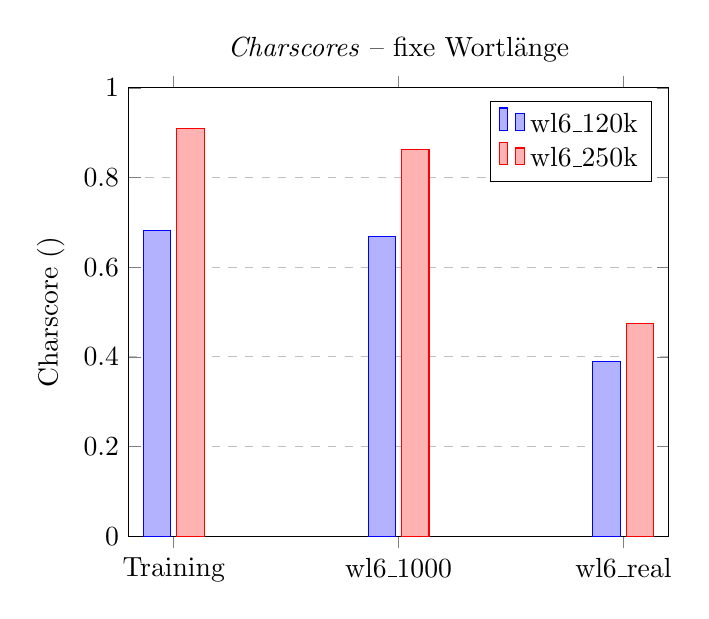
\begin{tikzpicture}
        \begin{axis}[
            title = {\textit{Charscores} -- fixe Wortlänge},
            ylabel = {Charscore ($\varnothing$)},
            ymin = 0, ymax = 1,
            ytick = {0, 0.2, 0.4, 0.6, 0.8, 1},
            ymajorgrids = true,
            grid style = dashed,
            legend pos = north east,
            symbolic x coords = {Training, wl6\_1000, wl6\_real},
            xtick = data,
            ybar
        ]

            \addplot coordinates {(Training, 0.6819) (wl6\_1000, 0.6685) (wl6\_real, 0.3889)};
            \addlegendentry{wl6\_120k};

            \addplot coordinates {(Training, 0.9086) (wl6\_1000, 0.863) (wl6\_real, 0.4753)};
            \addlegendentry{wl6\_250k};
        \end{axis}
    \end{tikzpicture}
    \caption{Charscores für verschiedene \textit{Trainings}-Datensatzgrößen\label{ergebnisse:scores:scoresviz}}
\end{figure}

\begin{figure}
    \centering
    \begin{tikzpicture}
        \begin{axis}[
            title = {Loss-Entwicklung für \texttt{wl6\_120k}},
            xlabel = {Epochen},
            ylabel = {Loss},
            xmin = 0, xmax = 24,
            ymin = 0, ymax = 11,
            xtick = {0, 3, 6, 9, 12, 15, 18, 21, 24},
            ytick = {0, 1, 2, 3, 4, 5, 6, 7, 8, 9, 10, 11},
            ymajorgrids = true,
            xmajorgrids = true,
            grid style = dashed,
            legend pos = north east,
            no markers
        ]

                \addplot table [x = epoch, y = loss, col sep = semicolon]{loss_120k.csv};
                \addlegendentry{loss};

                \addplot table [x = epoch, y = val_loss, col sep = semicolon]{loss_120k.csv};    
                \addlegendentry{val\_loss};
        \end{axis}
    \end{tikzpicture}

    \begin{tikzpicture}
        \begin{axis}[
            title = {Genauigkeitsentwicklung für \texttt{wl6\_120k}},
            xlabel = {Epochen},
            ylabel = {Genauigkeit},
            xmin = 0, xmax = 24,
            ymin = 0, ymax = 1.1,
            xtick = {0, 3, 6, 9, 12, 15, 18, 21, 24},
            ytick = {0, 0.1, 0.2, 0.3, 0.4, 0.5, 0.6, 0.7, 0.8, 0.9, 1},
            ymajorgrids = true,
            xmajorgrids = true,
            grid style = dashed,
            legend pos = south east,
            no markers
        ]

                \addplot table [x = epoch, y = acc, col sep = semicolon]{loss_120k.csv};
                \addlegendentry{acc};

                \addplot table [x = epoch, y = val_acc, col sep = semicolon]{loss_120k.csv};    
                \addlegendentry{val\_acc};
        \end{axis}
    \end{tikzpicture}
    \caption{Loss und Genauigkeit für den Datensatz \texttt{wl6\_120k}\label{ergebnisse:scores:loss120k}}
\end{figure}

\begin{figure}
    \centering
    \begin{tikzpicture}
        \begin{axis}[
            title = {Loss-Entwicklung für \texttt{wl6\_250k}},
            xlabel = {Epochen},
            ylabel = {Loss},
            xmin = 0, xmax = 24,
            ymin = 0, ymax = 9,
            xtick = {0, 3, 6, 9, 12, 15, 18, 21, 24},
            ytick = {0, 1, 2, 3, 4, 5, 6, 7, 8, 9},
            ymajorgrids = true,
            xmajorgrids = true,
            grid style = dashed,
            legend pos = north east,
            no markers
        ]

                \addplot table [x = epoch, y = loss, col sep = semicolon]{loss_250k.csv};
                \addlegendentry{loss};

                \addplot table [x = epoch, y = val_loss, col sep = semicolon]{loss_250k.csv};    
                \addlegendentry{val\_loss};
        \end{axis}
    \end{tikzpicture}

    \begin{tikzpicture}
        \begin{axis}[
            title = {Genauigkeitsentwicklung für \texttt{wl6\_250k}},
            xlabel = {Epochen},
            ylabel = {Genauigkeit},
            xmin = 0, xmax = 24,
            ymin = 0, ymax = 1.1,
            xtick = {0, 3, 6, 9, 12, 15, 18, 21, 24},
            ytick = {0, 0.1, 0.2, 0.3, 0.4, 0.5, 0.6, 0.7, 0.8, 0.9, 1},
            ymajorgrids = true,
            xmajorgrids = true,
            grid style = dashed,
            legend pos = south east,
            no markers
        ]

                \addplot table [x = epoch, y = acc, col sep = semicolon]{loss_250k.csv};
                \addlegendentry{acc};

                \addplot table [x = epoch, y = val_acc, col sep = semicolon]{loss_250k.csv};    
                \addlegendentry{val\_acc};
        \end{axis}
    \end{tikzpicture}
    \caption{Loss und Genauigkeit für den Datensatz \texttt{wl6\_250k}\label{ergebnisse:scores:loss250k}}
\end{figure}

\subsection{Performance}

Neben den erzielten Ergebnissen ist für die Nutzung auf einem HPC-System auch die Ausführungsgeschwindigkeit von
Interesse. Diese soll in den folgenden Abschnitten näher betrachtet werden.

\subsubsection{\textit{Training}}
\label{ergebnisse:performance:training}

Aufgrund der großen Datenmengen und der Komplexität des Netzwerks dauert das \textit{Training} -- abhängig vom konkreten
Datensatz -- wenige bis viele Stunden. Dabei zeigt sich, dass die Laufzeit proportional zur Größe des Datensatzes
ansteigt  (siehe Tabelle~\ref{ergebnisse:performance:training:laufzeit}).

\begin{table}
    \caption{\textit{Trainings}-Laufzeiten}
    \centering
    \begin{tabular}{|c|c|c|}
        \hline
        \textbf{Trainingsdatensatz} & \textbf{Gesamtlaufzeit} & \textbf{Epochenlaufzeit} \\ \hline \hline
        \texttt{wl6\_120k} & \SI{4}{\hour} \SI{20}{\minute} \SI{54}{\second} & \SI{10}{\min} \SI{39}{\second} \\ \hline
        \texttt{wl6\_250k} & \SI{9}{\hour} \SI{03}{\minute} \SI{22}{\second} & \SI{21}{\min} \SI{44}{\second} \\ \hline
    \end{tabular}
    \label{ergebnisse:performance:training:laufzeit}
\end{table}

\subsubsection{\textit{Inferenz}}

Bei der \textit{Inferenz} zeigt sich das gleiche Bild wie beim \textit{Training}. Auch hier steigt die Laufzeit
proportional zur Datenmenge an, fällt aber durch den geringeren Rechenaufwand deutlich kleiner aus als beim
\textit{Training} (siehe Tabelle~\ref{ergebnisse:performance:inferenz:laufzeit}).

\begin{table}[h]
    \caption{\textit{Inferenz}-Laufzeiten}
    \centering
    \begin{tabular}{|c|c|c|}
        \hline
        \textbf{Validierungsdatensatz} & \textbf{Gesamtlaufzeit} & \textbf{Laufzeit pro Bild}\\ \hline \hline
        \texttt{wl6\_120k} & \SI{19}{\minute} \SI{25}{\second} & \SI{9,7}{\milli\second} \\ \hline
        \texttt{wl6\_250k} & \SI{40}{\minute} \SI{17}{\second} & \SI{9,7}{\milli\second} \\ \hline
    \end{tabular}
    \label{ergebnisse:performance:inferenz:laufzeit}
\end{table}
